\documentclass[11pt,a4paper]{article}

\usepackage[utf8]{inputenc} 
\usepackage[T1]{fontenc} 
\usepackage{lmodern}
\usepackage[margin=2cm]{geometry}
\usepackage[german]{babel}
\usepackage{amsmath} 
\usepackage{graphicx} 
\usepackage{booktabs}
\usepackage{hyperref}
\hypersetup{
    colorlinks,
    citecolor=red,
    filecolor=black,
    linkcolor=black!20!blue!90!,
    urlcolor=black} 
\usepackage{nicefrac}
\usepackage[table]{xcolor}
\usepackage{tocloft}
\usepackage{array}

\newcolumntype{L}[1]{>{\centering\let\newline\\\arraybackslash\hspace{0pt}}m{#1}}

\setlength{\parindent}{0pt}
\setlength{\parskip}{1ex plus 0.5ex minus 0.5ex}

\definecolor{incolor}{rgb}{0.0, 0.0, 0.5}

\hbadness=99999

\newcommand{\refpy}[1]{Siehe Anhang: \textit{Rechnungen in Python} (\texttt{{\color{incolor}In [{\color{incolor}#1}]}})}
\newcommand\dif{\mathop{}\!\mathrm{d}}
\newcommand{\halftime}[4]{\begin{figure}[h]
\begin{minipage}{.#1\textwidth}#3\end{minipage}\begin{minipage}{.#2\textwidth}
\centering
#4\end{minipage}
\end{figure}}


\begin{document}


{
\centering 
\large 
Physiklabor für Anf\"anger*innen \\
Ferienpraktikum im Sommersemester 2018 \\[4mm]
\textbf{\LARGE 
Versuch 22: Kreisel
} \\[3mm]
(durchgef\"uhrt am 21.09.2018 bei Adrian Hauber) \\
Andréz Gockel, Patrick M\"unnich\\
\today \\[10mm]
}

\vspace{50pt}
\tableofcontents
\vspace{22pt}
\listoftables
\vspace{22pt}
\listoffigures
\pagebreak

\section{Ziel des Versuchs}
XXXX

\section{Teil XX}

\subsection{Theorie}

XXXX

\subsection{Aufbau}


\halftime{5}{5}{Es wurde ein Kreiselrad mit verstellbarer Kreiselachse verwendet. Dieser wurde auf ein Stativ mit einer drehbaren Halterung die es ermöglichte eine Präzessionsbewegung zu durchlaufen. Eine Federwaage wurde verwendet um die Masse des Kreisels zu bestimmen. Es wurden zwei Stoppuhren benutzt um jeweils die Präzessionsfrequenz und die Rotationsfrequenz zu messen. 
}{\fbox{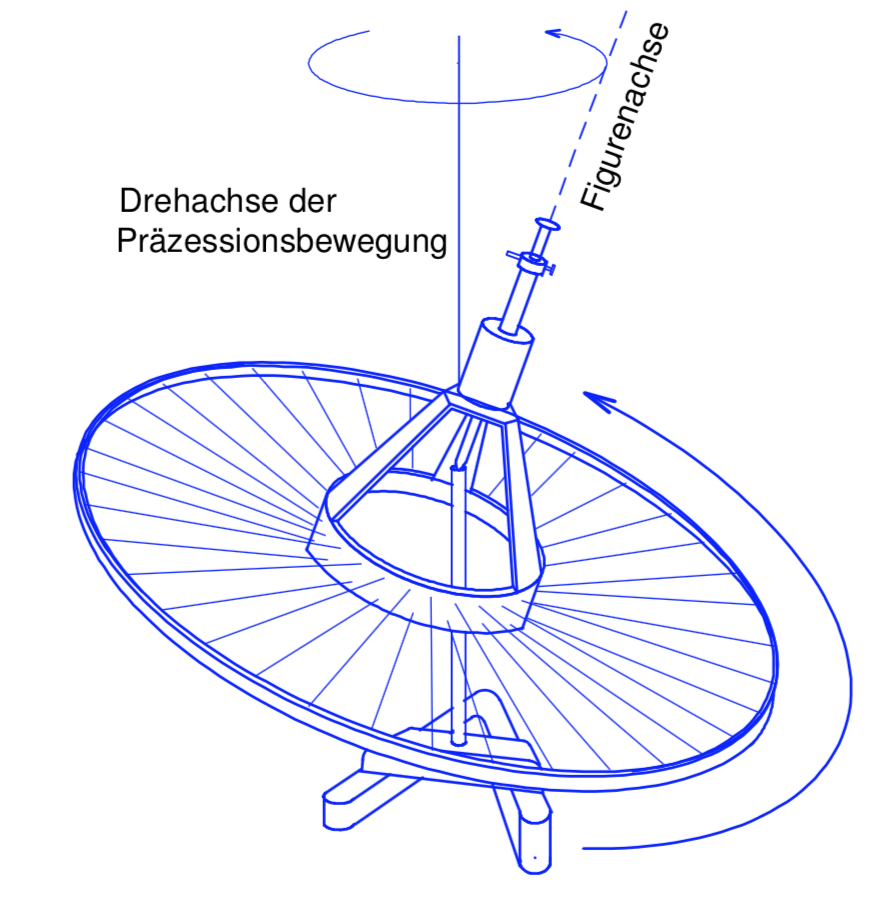
\includegraphics[width=0.9\textwidth]{Krpr}}
   \renewcommand\thefigure{B1}
\caption[Präzessierender Kreisel]{Präzessierender Kreisel \cite{Anleitung}}
\label{Pic:1}}

\subsection{Durchführung}

Zuerst wurde Masse des Kreisels gemessen. Zunächst wurde die Kreiselachse eingestellt, dann wurde das Kreiselrad angehoben und per hand im Uhrzeigersinn gedreht. Der rotierende Kreisel wurde dann vorsichtig auf die Halterung platziert und gekippt. Dann wurden 10 Rotationen zeitlich gemessen, und eine Präzessionsbewegung. Dies wurde für 10 verschiedene Kreiselachsen vier mal durchgeführt. Die Drehrichtung der Präzessionsbewegung wurde jedesmal notiert. Es konnten nur die Drehrichtung bestimmt werden für die Einstellungen wo der Schwerpunkt zu nahe dem Unterstützungspunkt war.

\subsection{Auswertung}

XXXX

\section{Diskussion}

XXXX

\pagebreak

\section{Anhang: Tabellen und Diagramme}

\begin{table}[h]
\centering
\caption{Messwerte} \vspace{11pt}
$\begin{array}{l}
\textrm{Unsicherheiten:}\\
\textrm{Zeit: } \pm 0.3 \textrm{s}\\
\textrm{Länge: } \pm 0.05 \textrm{cm}\\
\end{array}$
\begin{tabular}{ r L{3cm} L{3cm} }
\toprule
$l$\textrm{ in cm} & \textrm{Präzession umlaufdauer\textrm{ in s}} & \textrm{10 Rotationen umlaufdauer}\textrm{ in s} \\
\midrule
1 & 6.6 & 5.1\\
1 & 4.7 & 6.9\\
1 & 3.6 & 8.1\\
1 & 7.9 & 4.2\\
\hline
2 & 6.5 & \phantom{0}6.7\\
2 & 6.7 & \phantom{0}6.7\\
2 & 7.0 & 13.7\\
2 & 9.4 & \phantom{0}5.5\\
\hline
3 & 13.7 & 6.8\\
3 & 14.4 & 6.2\\
3 & \phantom{0}9.8 & 7.8\\
3 & 13.4 & 6.1\\
\hline
8 & 5.7 & 6.4\\
8 & 6.6 & 5.5\\
8 & 5.6 & 6.6\\
8 & 6.4 & 6.0\\
\hline
9 & 5.1 & 5.7\\
9 & 4.7 & 6.5\\
9 & 4.1 & 8.0\\
9 & 6.3 & 4.5\\
\hline
10 & 1.7 & 6.7\\
10 & 2.7 & 5.0\\
10 & 3.9 & 3.6\\
10 & 3.2 & 4.0\\
\bottomrule
\end{tabular}
\phantom{$\begin{array}{l}
\textrm{Unsicherheiten:}\\
\textrm{XXXX: } \pm XX \textrm{XX}\\
\end{array}$}
\label{Tab:X}
\end{table}

\begin{figure}[p]
\centering
\fbox{\includegraphics[width=0.8\textwidth]{NAME}}
\renewcommand\thefigure{BX}
\caption[XXXX]{XXXX}
\label{Abb:X}
\end{figure}

\begin{thebibliography}{9}
\bibitem{Uncertainties}''Correlations between variables are automatically handled, which sets this module apart from many existing error propagation codes.'' - https://pythonhosted.org/uncertainties/
\bibitem{Anleitung} Physikalisches Institut der Albert-Ludwigs-Universität Freiburg (Hrsg.) (08/2018): Versuchsanleitungen zum Physiklabor für Anfänger*innen, Teil 1, Ferienpraktikum im Sommersemester 2018.
\end{thebibliography}

\end{document}